% !TEX TS-program = pdflatex
% !TEX encoding = UTF-8 Unicode

% Author: Michael Wagener

\documentclass[11pt]{article} % use larger type; default would be 10pt

\usepackage{pgf}
\usepackage{tikz}
\usetikzlibrary{arrows,automata,shapes}
\usetikzlibrary{decorations.pathmorphing} % LATEX and plain TEX when using Tik Z

\usepackage[utf8]{inputenc} % set input encoding (not needed with XeLaTeX)
\usepackage{geometry} % to change the page dimensions
\geometry{a4paper} % or letterpaper (US) or a5paper or....
\geometry{margin=15mm} % for example, change the margins to 2 inches all round
%\usepackage[ngerman]{babel}

\usepackage{booktabs} % for much better looking tables
\usepackage{array} % for better arrays (eg matrices) in maths
\usepackage{paralist} % very flexible & customisable lists (eg. enumerate/itemize, etc.)
\usepackage{verbatim} % adds environment for commenting out blocks of text & for better verbatim
\usepackage{subfig} % make it possible to include more than one captioned figure/table in a single float
\usepackage{listings}
\usepackage[obeyspaces,spaces]{url} % https://tex.stackexchange.com/questions/164446/how-to-typeset-a-file-path

\usepackage{float}  % https://en.wikibooks.org/wiki/LaTeX/Floats,_Figures_and_Captions
%\floatstyle{boxed} 
\restylefloat{figure}

\usepackage{graphicx}  % https://www.namsu.de/Extra/pakete/Wrapfig.html
\usepackage{wrapfig}   % https://mirror.clientvps.com/CTAN/macros/latex/contrib/wrapfig/wrapfig-doc.pdf

\usepackage{scrextend} % für addmargin
\usepackage{color}
\definecolor{mark}{rgb}{0.8,0.2,0.2} % 1=weiß, 0=schwarz
\definecolor{rowcolor}{rgb}{0.94, 0.97, 1.00}
\definecolor{rowkeycol}{rgb}{0.99, 0.97, 0.80}

\author{Michael Wagener, JCNS-1}
\title{SAS Scatter2 \\[1ex] {\large User documentation}}

\usepackage{fancyhdr} % This should be set AFTER setting up the page geometry
\pagestyle{fancy} % options: empty , plain , fancy
\renewcommand{\headrulewidth}{0pt} % customise the layout...
\lhead{}\chead{\textbf{SAS Scatter2 Calculations}}\rhead{\today}
\lfoot{Michael Wagener}\cfoot{\thepage}\rfoot{JCNS-1}

\usepackage{sectsty}
\allsectionsfont{\sffamily\mdseries\upshape} % (See the fntguide.pdf for font help)
% (This matches ConTeXt defaults)

%%% ToC (table of contents) APPEARANCE
\usepackage[nottoc,notlof,notlot]{tocbibind} % Put the bibliography in the ToC
\usepackage[titles,subfigure]{tocloft} % Alter the style of the Table of Contents
\renewcommand{\cftsecfont}{\rmfamily\mdseries\upshape}
\renewcommand{\cftsecpagefont}{\rmfamily\mdseries\upshape} % No bold!

\usepackage{longtable} % Tabellen über mehrere Seiten
\usepackage{multirow} % multirow/multicolumn
\usepackage{colortbl} % farbige Tabellenzellen
%\setlength{\LTpre}{0pt} % Remove whitespace befor and after longtables
%\setlength{\LTpost}{0pt}

\usepackage{tabularx}
\newcolumntype{L}[1]{>{\raggedright\arraybackslash}p{#1}} % linksbündig mit Breitenangabe
\newcolumntype{C}[1]{>{\centering\arraybackslash}p{#1}} % zentriert mit Breitenangabe
\newcolumntype{R}[1]{>{\raggedleft\arraybackslash}p{#1}} % rechtsbündig mit Breitenangabe
\newcommand{\ltab}{\raggedright\arraybackslash} % Tabellenabschnitt linksbündig
\newcommand{\ctab}{\centering\arraybackslash} % Tabellenabschnitt zentriert
\newcommand{\rtab}{\raggedleft\arraybackslash} % Tabellenabschnitt rechtsbündig
% https://de.wikibooks.org/wiki/LaTeX-W%C3%B6rterbuch:_tabular

\usepackage[colorlinks, linkcolor = black, citecolor = black, filecolor = black, urlcolor = blue]{hyperref}
% https://de.wikibooks.org/wiki/LaTeX-W%C3%B6rterbuch:_hyperref


\setlength{\tabcolsep}{1mm} % Setzt den Längenwert von {Abstand zwischen den Spalten einer Tabelle} auf den Wert 1mm
\setcounter{tocdepth}{3} % Tiefe des Inhaltsverzeichnisses

\begin{document}

\maketitle
\tableofcontents % toc anzeigen

\clearpage
\begin{figure}  % [b] % die History Tabelle am unteren[b] Seitenrand der ersten Seite anzeigen...
% Da das Inhaltsverzeichnis größer geworden ist, wird diese jetzt auf der zweiten Seite platziert.
\begin{longtable}{|p{2.7cm}|p{2.6cm}|p{10.3cm}|}
\caption{Document revision history} \\
\hline\rowcolor{rowcolor}{\bf Date} & {\bf Author} & {\bf Short description} \\
\endfirsthead
\hline
03. Dec 2021 & M.Wagener & Start with a copy of a former version. \\ \hline
%18. Jan 2022 & M.Wagener & Continue writing and insert screenshots. \\ \hline
%04. Feb 2022 & M.Wagener & Finish chapter 2 and start with chapter 3. \\ \hline
04. Mar 2022 & M.Wagener & Add directory infos of the git and work on the AI part. \\ \hline
08. Dec 2022 & M.Wagener & Upload to github (under the name CrystalScatter). \\ \hline
12. Jun 2023 & M.Wagener & Start writing about the GUI-Redesign. \\ \hline
22. Jun 2023 & M.Wagener & Finish the first version after GUI-Redesign. \\ \hline
27. Jun 2024 & M.Wagener & Update screenshots and some descriptions, add Chatbot. \\ \hline
\end{longtable}

\centerline{All sources saved at https://iffgit.fz-juelich.de/wagener/sas-crystal (only private access)}
\centerline{Snapshots on \url{https://github.com/neutron-simlab/CrystalScatter} with global access}
\end{figure}

\clearpage % neue Seite beginnen


\section{Preface}

The request was to convert a Pascal program for crystal calculations\footnote{Executable download not working anymore, please contact s.foerster@fz-juelich.de}
%from http://www.bzkg.uni-bayreuth.de/de/download/index.html}
to a usable C++ routine and run it faster with the help of a GPU.

If you are interested in the mathematical backgrounds, please see the nature scientific report \\
\centerline{\it Fast calculation of scattering patterns using hypergeometric function algorithms}
\centerline{\url{https://www.nature.com/articles/s41598-023-27558-8}} \\

During the development the GUI and the internals were changed more than once. But now the system becomes better and seems to be useful, so I marked it with the number {\it 2} in the name. This documentation address the users, another documentation will be written for developers to explain some internals. All internals are documented inline.

The software is written with the Qt library, so that it can run under windows and linux without changes in the source. {\it Due to the used compiler, a GPU cannot be used under Windows.} All screenshots are made on a windows system. It is possible that some parts of the screenshots differs from the current look of the program, it will be developed and the screenshots are not updated every time.

\subsection{Installation and usage hints}

The program can be used under different systems:
\begin{itemize}\itemsep0pt
\item {\bf Windows} (Standalone) \\
	the program can be compiled as one executable file for Windows (10 or later, 64bit). This can be used on your local system without any other software installed.
\item {\bf Windows} (from source) \\
	{\bf Linux} (from source) \\
	{\bf MacOS} (from source) \\
	you can get access to the git system, where the source is available. Then you have to install the Qt development environment and some other libraries\footnote{{\bf FFTW3} for FFTs, if installed this replaces a simple internal code. {\bf HDF5} to read this datatype} if you need the functionality. Then you can compile this program and use it.
\item {\bf Android} (Tablet) \\
	it is possible to compile the program for Android and run it on a tablet computer. This makes only sense if the tablet has more than 4 cores and the cpu is fast.
\item {\bf IOS} (Tablet) \\
	at the moment I'm not able to compile for the IOS system.
\end{itemize}

\clearpage
\section{GUI}

After the start of the program you get this screen. In the upper right corner is the current version number and the release date.

\begin{figure}[H]
 \centering
 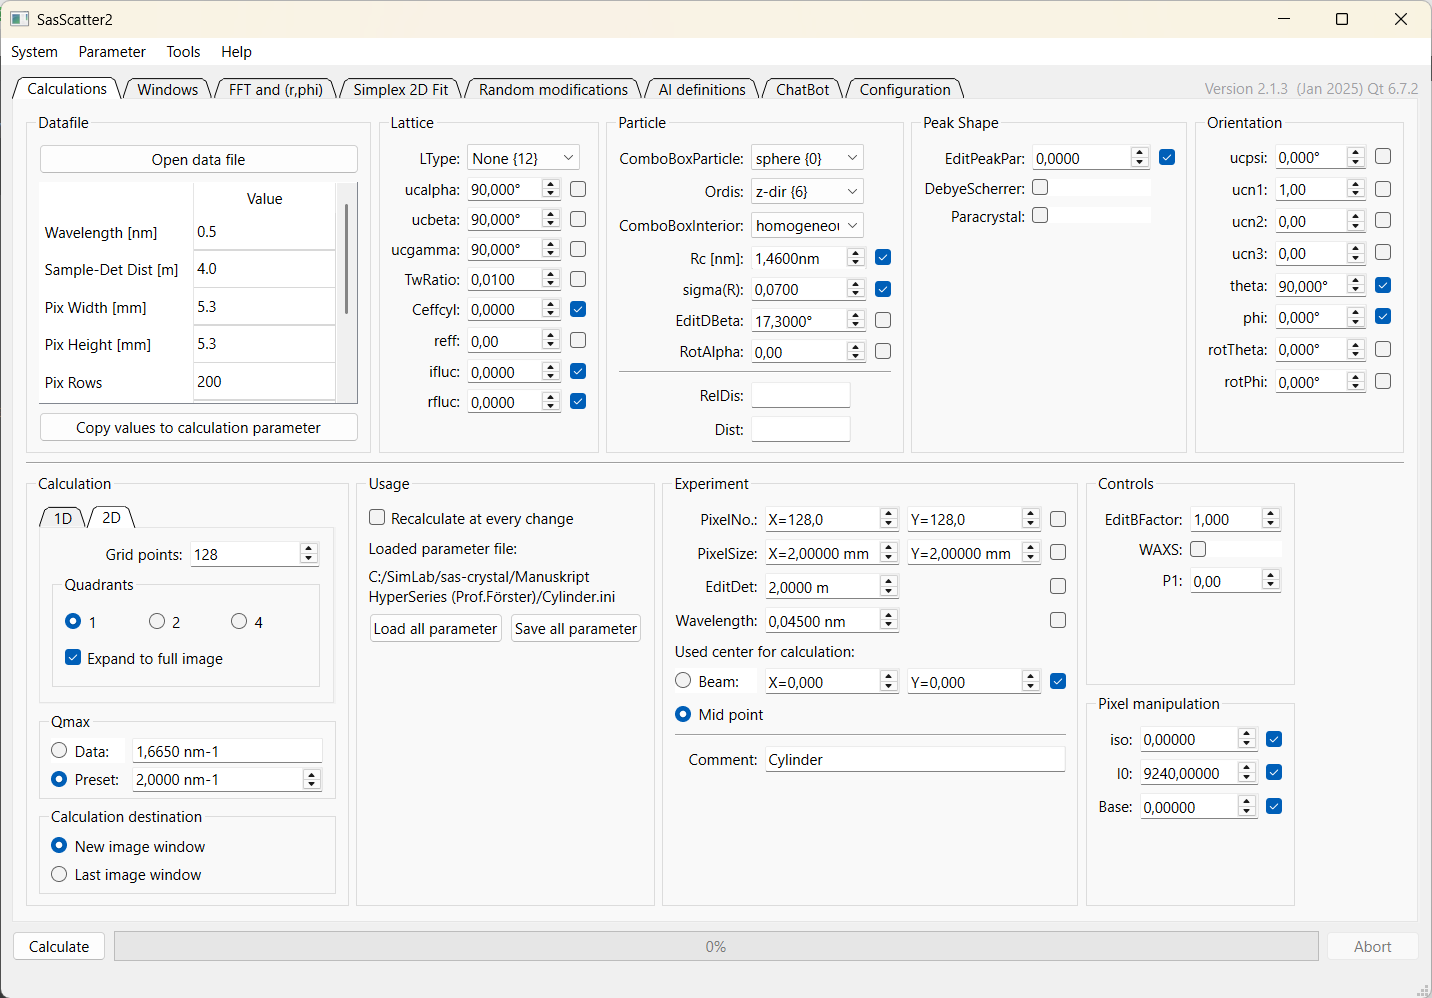
\includegraphics[width=\textwidth]{gui-calculations.png}
 \caption{Calculation parameter overview after startup.}
% \label{fig:calcstart}
\end{figure}
Now we go through all parts of this gui.


\subsection{Menubar}

the menubar on the top has four parts.

\subsubsection{System}

%\begin{wrapfigure}{r}{0.09\textwidth}
%  \begin{center}
%    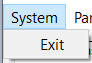
\includegraphics[width=0.08\textwidth]{menu-system.png}
%  \end{center}
% %\caption{System menu}
% %\label{fig:menusys}
%\end{wrapfigure}
This system menu contains only the {\it Exit} function. But the Window-Closebutton can be used also to exit the program. If you want to exit the program during a calculation, the program can crash, but this doesn't matter in this case.

\subsubsection{Parameter}

\begin{wrapfigure}{r}{0.33\textwidth}
  \begin{center}
    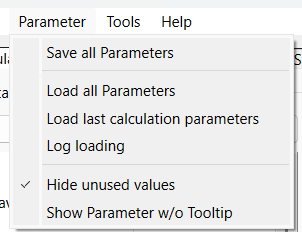
\includegraphics[width=0.27\textwidth]{menu-parameter.png}
  \end{center}
 %\caption{System menu}
 %\label{fig:menusys}
\end{wrapfigure}
With this parameter menu the user can load and save the current calculation parameters. The save asks allways for a filename. Just before a calculation starts, all parameters are saved into a special file and this file can be loaded with the {\it Load last calculation parameters}.

The menu topic {\it Hide unused values} can be toggled. If it is set, all parameters not used in the current calculation are hidden completly. If this is not set, then all unused parameters are shown with a disabled label and fit-checkbox, but the values are changable.
\\

\subsubsection{Tools}

\begin{wrapfigure}{r}{0.31\textwidth}
  \begin{center}
    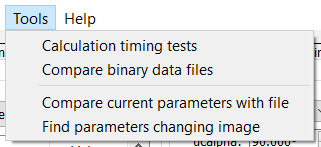
\includegraphics[width=0.30\textwidth]{menu-tools.png}
  \end{center}
 %\caption{System menu}
 %\label{fig:menusys}
\end{wrapfigure}
There are some tools implemented, mostly as an answer to development questions as a help function.
\begin{itemize}\itemsep0pt
\item {\it Calculation timing tests} - can be used for some benchmarking and will be described later in this document.
\item {\it Compare binary data files} - this will compare two data files saved with this program. These files contains the dimensions (first 20 characters) and then the image in binary representation.
\item {\it Compare current parameters with file} - this will compare all current parameters with the informations read from a parameter file. All different parameters are highlighted with a green background and the value from the file is put in the tooltip text for this parameter.
\item {\it Find parameters changing image} - all parameters (except the size informations) will be checked if they are changing the binary image. For this the current image is calculated and saved in memory, then each parameter ist changed +10\% and -10\% and each time the calculated image is compared with the starting image. Each parameter with a change will be highlighted with a cyan background.
\item {\it Start autoprocessing file} - this will select a file with some commands and process them. Then this file can be used to be automatically processed at program start if given as a command line parameter.
\end{itemize}
If one colored background is set, an explanation for the colors is displayed in the Usage group box.

\subsubsection{Help}

%\begin{wrapfigure}{r}{0.20\textwidth}
%  \begin{center}
%    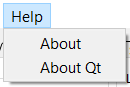
\includegraphics[width=0.14\textwidth]{menu-help.png}
%  \end{center}
% %\caption{System menu}
% %\label{fig:menusys}
%\end{wrapfigure}
\begin{itemize}\itemsep0pt
\item {\it About} - shows the authors and some other informations.
\item {\it About Qt} - shows a predefined message from the Qt Library.
\end{itemize}


%\clearpage
\subsection{The calculation button and progress bar}

Just below the menu bar some tabs can be selected. They group the functions of this program. The following chapters will describe each of these functions, starting with a screenshot of the window.

At the bottom left of this GUI is the button to start the calculation of the current simulation image. The progress bar shows the calculation progress. If the calculation is performed on the CPU, it can be aborted with the button on the right. If you click the abort button, the calculation threads will be terminated but it can take some seconds until the threads will stop and the image window is shown\footnote{Sometimes it is possible that the program crashed at this point. I didn't know why but I'll work on it.}. The same procedure is used to stop the calculation after a specified time limit (see Configuration tab).

If the calculation is performed on the GPU, the abort button will be disabled because this function is not available.


\clearpage
\subsection{Main area tabs}

\subsubsection{Calculations}
\begin{figure}[H]
 \centering
 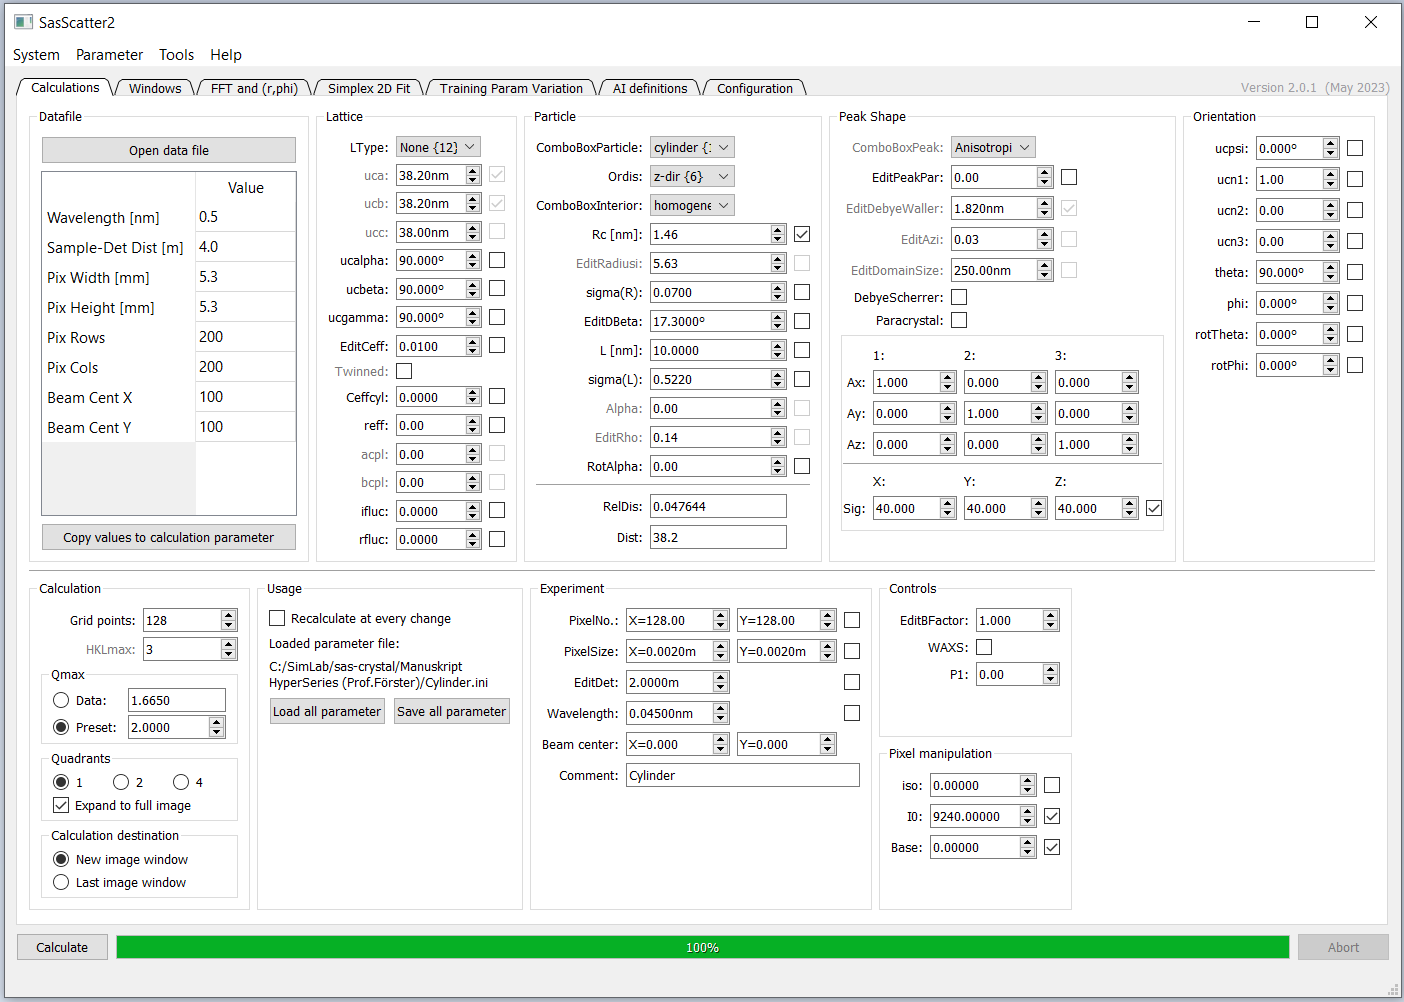
\includegraphics[width=\textwidth]{gui-calculations-nohidden.png}
 \caption{Calculation parameter with no hidden values.}
\end{figure}

All data inputs are logically grouped. On the right of most input fields there is a check box. If this box is checked, this parameter will be used during the simplex 2d fit operation described later in this document.
\begin{itemize}\itemsep0pt
\item Group {\it Datafile} - here you can open a data file from real measurements for the fit algorithm. You can select different data types (by file extensions), the data is loaded and displayed in a new image window. All known header informations are stored in the meta informations of the image window. If available, some specified informations from the data file header are displayed below this button. You can copy these values into the desired fields for the calculation with one click. The possible data file formats are:
	\begin{itemize}\itemsep0pt
	\item TIFF-Images (*.tif *.tiff), multiple images are not recognized in the current version
	\item KWS-Data (*.dat *.data)
	\item ESRF/Klora images (*.edf), might be very large
	\item Spreadsheet-Format (*.spr)
	\item 2D SANS (*.xml *.csv *.dat)
	\item SasCrystal (*.dat *.csv *.txt), the local format if images are saved
	\item[] {\it If the HDF5 library is included:}
	\item HDF5 Files (*.h5 *.hdf *.hdf5 *.nxs), if more than one image is found, a selection dialog will ask the user which image(s) should be loaded and displayed. If used in the automatic fit, only the first selected image will be used. {\it The meta data usage is under development.}
	\end{itemize}
\item Group {\it Lattice} - select the lattice type and set the useful parameters for the calculations.
\item Group {\it Particle} - set the used particle type and the calculation parameters. The two values at the lower part of this group are output values calculated during the run.
\item Group {\it Peak Shape} - here you can define the peak shape parameters. The lower 3 by 3 values define the peak shape directions and the last three values are the domain size values for each axis.
\item Group {\it Orientation} - these are the orientation and rotation of the sample.
\item Group {\it Calculation}
	\begin{itemize}\itemsep0pt
	\item Grid points: number of pixel of one quadrant of the generated image. The 128 in the screenshot results in an image of 256*256 pixel.
	\item HKLmax: defines the number of calculation iterations and has a significant effect on the calculation time.
	\item Qmax: this sets the image dimension in Q-range and can be changed between the value calculated from the data file or the value entered by the user.
	\item Quadrants: here you can select, if only one quadrant(1) or the half(2) of the image or the full image(4) are calculated. If the checkbox {\it Expand to full image} is checked, the rest of the image is mirrored over the center to generate allways a full image. This is only usefull if the beam center ist set to zero.
	\item Calculation destination: here you can select if the calculated image will be shown in a new window or to overwrite the last image window. This is the same information as in the Configuration tab.
	\end{itemize}
\item Group {\it Usage} - if the recalculate checkbox is checked, every value change in the other fields starts a calculation. If the calculation is longer than 2 seconds, this box is unchecked. Below this the current loaded parameter file is shown and you can load / save the parameters in the same way as from the menu bar. If some input fields are marked with a colored background a short explanation will be displayed here too.
\item Group {\it Experiment} - the pixel dimensions and the size of the detector, the distance from sample to detector, the used wavelength and the x and y pixel position in the grid (one quarter of the result image) of the beam center. The comment field text is displayed in the image window.
\item Group {\it Controls} - some control factors for the calculation.
\item Group {\it Pixel manipulation} - the base is added to each pixel value. The iso value is multiplied with the calculated iso portion of the pixel value and then added to the normal value before multiplying with the I0 value.
\end{itemize}


\subsubsection{Windows}
\begin{figure}[H]
 \centering
 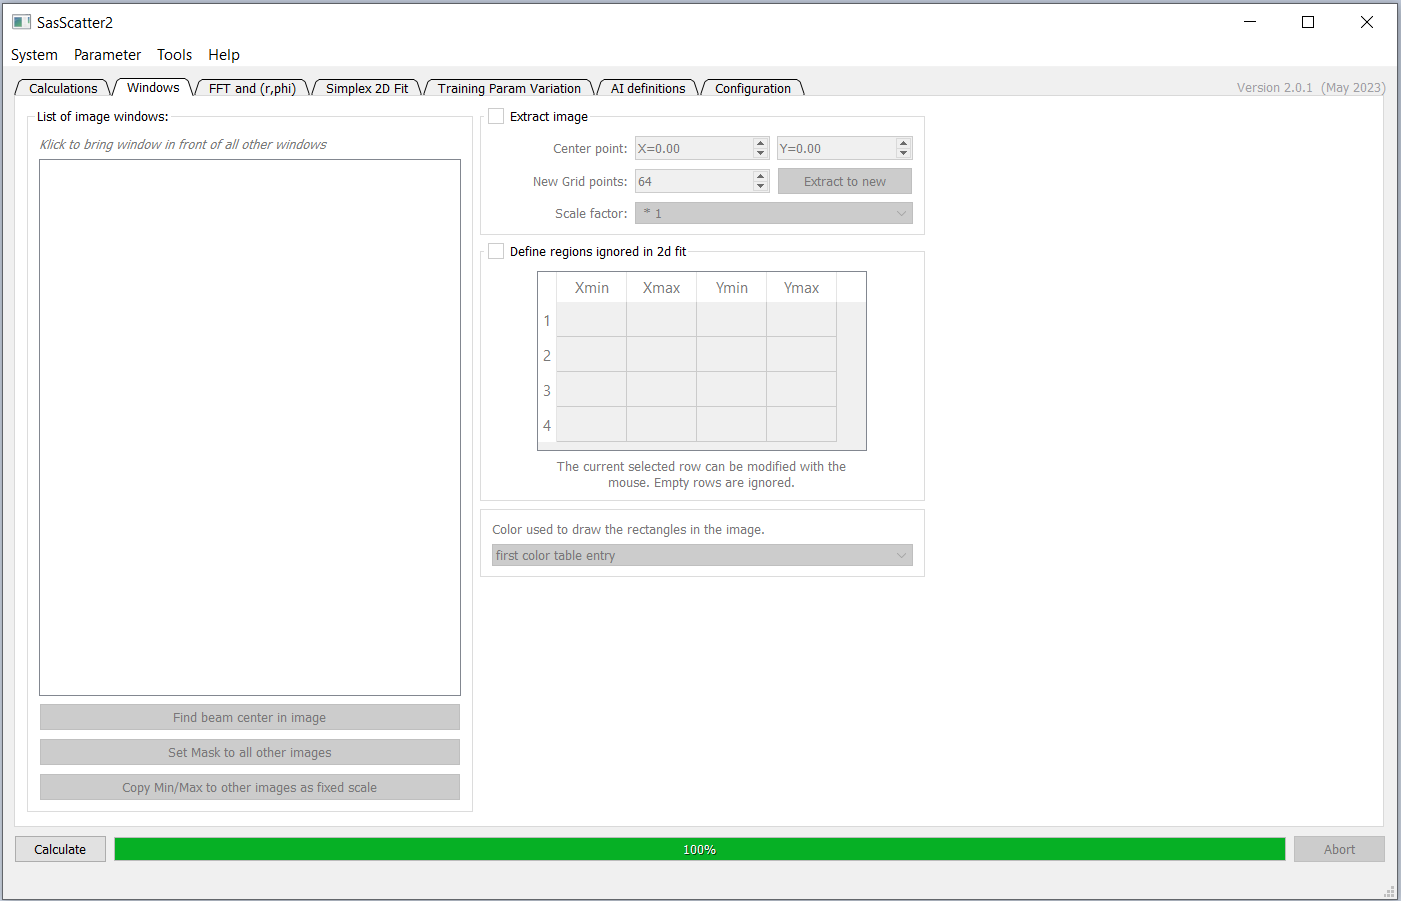
\includegraphics[width=\textwidth]{gui-windows.png}
 \caption{Window options}
\end{figure}

On the left a list with all image windows is shown and a click on an entry rises the image window on top of all other windows. So you can find them.
\begin{itemize}\itemsep0pt
\item Button {\it Find beam center in image} \\
	All KWS images have {\it zero pixels} at the corners and at the beam center. The pixel in the middle are searched and the middle point of this region is the beam center. This point can be used for further calculations.
\item Button {\it Set Mask to all other images} (enabled if more than one image window is open) \\
	This will generate a new image for each of the images in the list not selected. The image will be taken from the original image but all pixel where the KWS image has zeros, are set to zero.
\item Button {\it Copy Min/Max to other images as fixed scale} (enabled if more than one image window is open) \\
	Most times the image scaling will be logarithmic. So it is not so easy to compare images visually if they have different linear min / max values. With this option the scaling of the selected image is copied to all other images as a fixed scaling so that all images have the same visual scaling.
\end{itemize}

The following parts in the middle are enabled if one image window is activated in the left list. All drawings are done in this image.

The {\it Extract image} group can be checked. Then you can click and draw a square frame in this image. This region is described with the center point and the size here for fine adjustments. Then you can extract this region into a new image window.

In the same way you can define up to 4 regions which are ignored during the 2d fit. For this activate the group {\it Define regions ignored in 2d fit}, click in one row in the table and draw this rectangular region in the image window. If you want, you can enter the numbers manually in this table. These values are saved between program runs.

To modify the colour of the line drawing the regions, you can select it to 

First color table entry, Last color table entry, Red, White



\subsubsection{FFT and (r,phi)}
\begin{figure}[H]
 \centering
 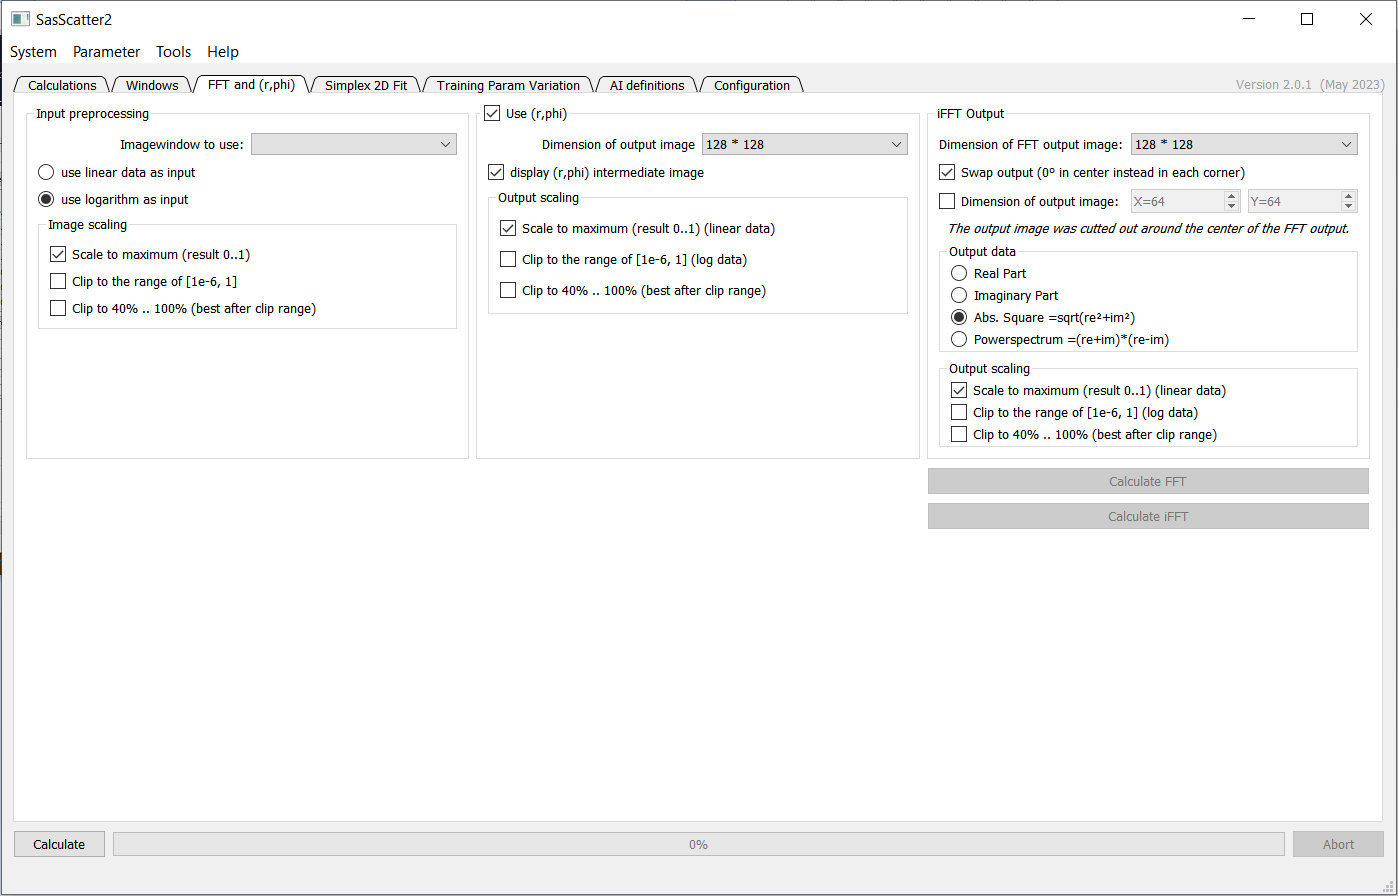
\includegraphics[width=\textwidth]{gui-fft.png}
 \caption{Image postprocessing options}
\end{figure}

This postprocessing can be done manually after the calculation of an image or it can be used during image generation for AI (see the AI definition tab). If enabled, a (r,phi) image is calculated from the input image. From this intermediate image or the original image  the normal or inverse FFT will be calculated. The options in this screen are:
\begin{itemize}\itemsep0pt
\item Group {\it Input preprocessing}: \\
	First you have to select the input image window. 
	It is possible to use the image data as is (linear) or calculate the logarithm first. 
	And you can select the image scaling (see below).
\item Group {\it Use (r,phi)}, if checked you can: \\
	Select the size of the output image (only dimensions of $2^n$ allowed). 
	Select if the intermediate (r,phi) image will be displayed. 
	And you can choose the output scaling (see below).
\item Group {\it iFFT Output} \\
	First select the size of the calculated FFT image (only dimensions of $2^n$ allowed). 
	The output can be swapped so that the zero is in the center and not at the corners as usual. 
	You can crop a region around the center as the resultant output. This might be better in scaling. 
	Select one of the possible FFT output functions. 
	And you can choose the output scaling (see below).
\item Calculate FFT / iFFT \\
	These buttons will start the calulation.
\end{itemize}

The output scaling groups can scale the image to the maximum or you can clip the image to the range $10^{-6}$ to 1. After this you can clip the image to the range of 40\% to 100\%. Or you can deselect all and do nothing.


\subsubsection{Simplex 2D Fit}
\begin{figure}[H]
 \centering
 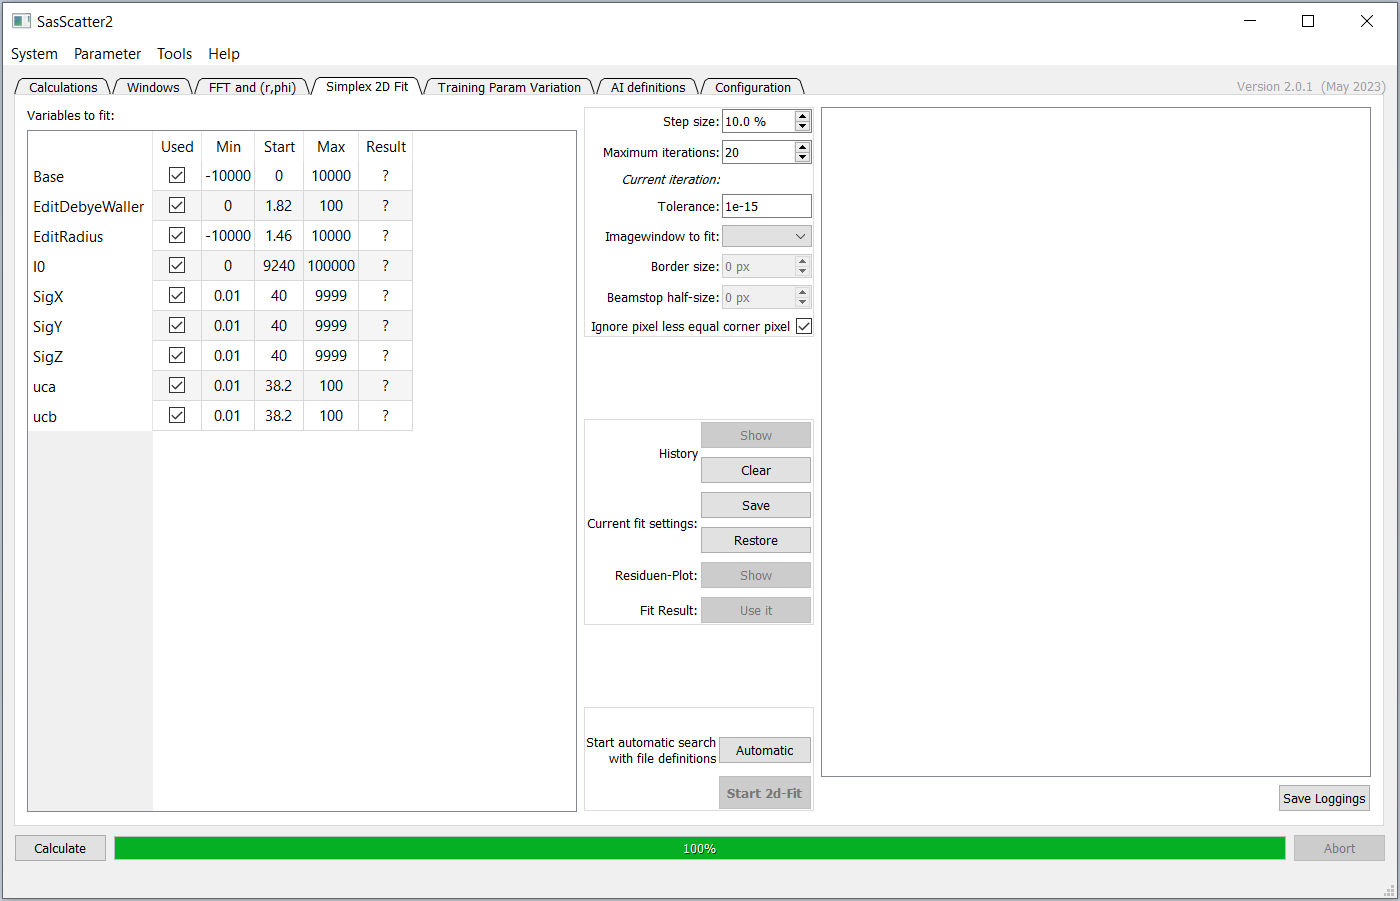
\includegraphics[width=\textwidth]{gui-fit.png}
 \caption{Simplex 2D Fit}
\end{figure}

To optimize the parameters a {\it Downhill Simplex 2d Fit} algorithm is implemented. It can be started manually in this tab and can work in an automatic mode (described later).

The left list contains all possible fitable parameters. They have checked checkboxes in the Calculation tab. {\it Due to the internal data structures the maximum number of variables is limited to 30.} For each parameter in this list you can:
\begin{itemize}\itemsep0pt
\item select if this parameter is used for the fit algorithm
\item set the min and max values as the fit limits
\item set the start value for the fit
\item view the result of the last fit run (last column)
\end{itemize}

The list at the right is filled during the fit process if the update flag in the configuration tab is checked. All messages are allways written in a temporary file which might be saved for future use with the button below the list.

The options in the middle are:
\begin{itemize}\itemsep0pt
\item {\it Step size}: is used to calculate the next values during the fit.
\item {\it Maximum iterations}: is the limit of the fit iterations if the tolerance is not reached.
\item {\it Tolerance}: is the maximum limit of the sum of squared errors.
\item {\it Imagewindow to fit}: is to select which image to be fitted.
\item {\it Border size}: is the number of pixel to be ignored during the fit at each border.
\item {\it Beamstop half size}: is the number of pixel to be ignored around the beam stop.
\item {\it Ignore pixel less equal corner pixel}: if checked, the pixel values above are disabled and all pixel less or equal the corner (first data value) are ignored during the fit. This is often usefull for KWS images.
\item {\it History}: This internal trend table contains all used parameters with all values after each run. It can be printed out ({\it Show}) on the console and {\it Clear}ed. In the automatic mode this table can be saved in the \LaTeX\ output file.
\item {\it Current fit settings}: the current values in the left list can be saved and reloaded. This is only stored in one memory location, so only one set of values can be saved. The next save overwrites the one before.
\item {\it Residuen Plot}\footnote{This feature is experimental}: this shows a new image with the differences between the original image and the last fit. The negative values are in greyscale and the positive values are in glowing or temperature color tables.
\item {\it Fit result}: sets the current result values as new start values in the calculation tab and in the current settings. After this simply click the Calculate button in the lower left corner and get an image with the fit result.
\item {\it Start automatic}: here you can select a file and some optione (see below) to start the automatic fit process. The file format is described later.
\item {\it Start 2d-Fit}: button starts one fit run with the current settings and displays the result values in the list. No image window will be generated.
\end{itemize}

\begin{wrapfigure}{r}{0.51\textwidth}
  \begin{center}
    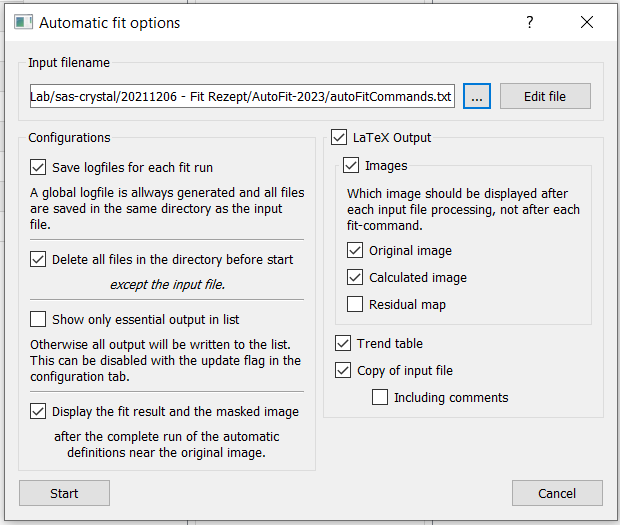
\includegraphics[width=0.5\textwidth]{gui-fit-auto.png}
  \end{center}
  \caption{Automatic fit configuration}
\end{wrapfigure}
In this automatic fit configuration dialog you can select the input file for the automatic fit and set some ouptions for the generated output. All informations are saved if the start button is clicked. This will start the automatic fit operation.

The most detailed option part is for the \LaTeX\  output file generated. Even if the images are not included in the file, the image files are generated. The Trend table contains all used parameters with all values after each fit run. The input commands can be included in the \LaTeX\  output. It is possible that some characters in the commentlines of the input file can confuse the \LaTeX\ converter, so you can exclude the comments for the output file.

During the fit operations all informations can be saved in special files if the {\it Save logfiles} is checked. One global logfile is generated if the command is included in the command file. The {\it Delete all files} checkbox can be used to delete all files except the input file before the fit run starts. With the {\it Show only essential output in list} you can reduce the amount of output in the list to speed up if logged in via network. If you want to show the result immediately after the run, you can check the {\it Display the fit result and the masked image}.


\clearpage
\subsubsection{Random modifications}
\begin{figure}[H]
 \centering
 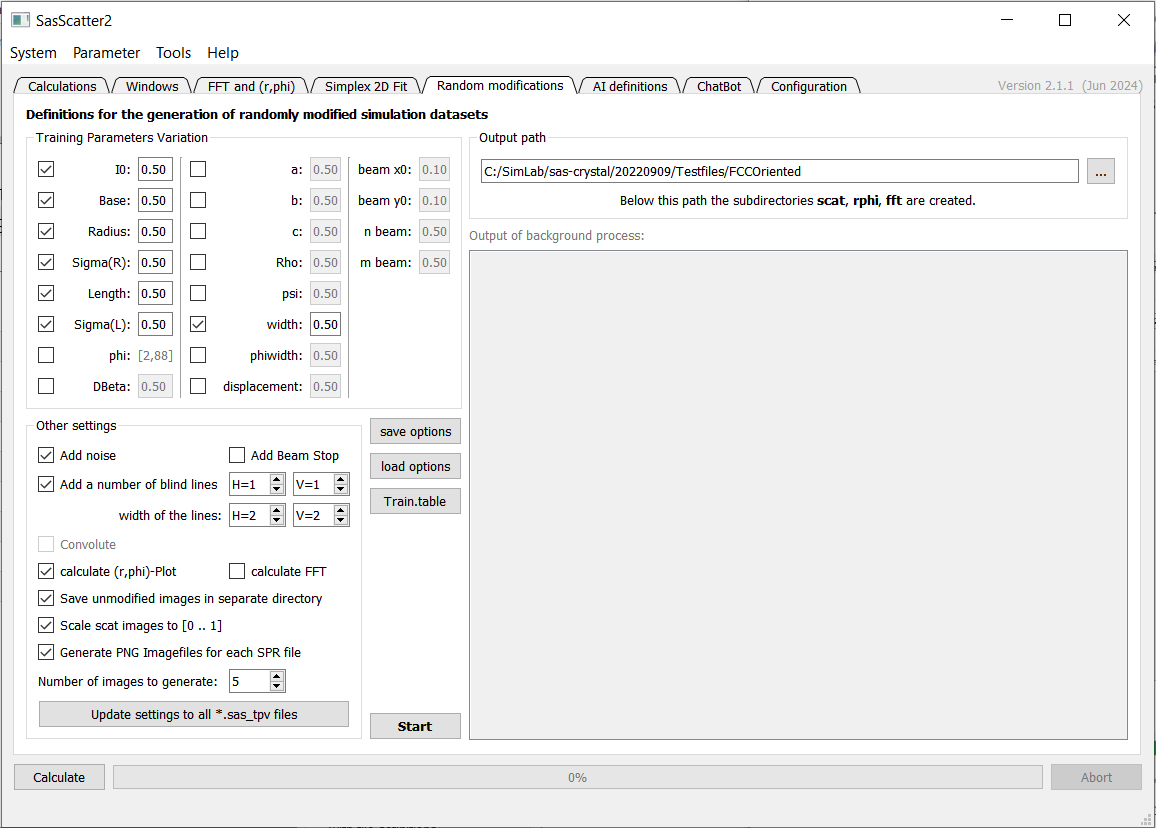
\includegraphics[width=\textwidth]{gui-tpv.png}
 \caption{Random modifications}
\end{figure}

In this tab you can generate a sequence of images comparable with the AI sequence explained below. The differences are (1) that you have here less manipulation features and (2) all images are saved in SPR-Format.

In the group {\it Training Parameters Variation} you can select which parameter should be used and a factor (0.01 to 1.00). Each image is then calculated with the selected parameters generated as: \\
\centerline{$current = 1 + paramvalue * factor * zuf$}
where {\it current} is the used value for the calculation, {\it paramvalue} is the value from the Calculation tab (or the parameter file), {\it factor} is the given factor in the range from 0.01 to 1.00 and {\it zuf} is a random number in the range from -1 to +1. The only exception is the value of {\it phi}, this is a random value in the range from 2 to 88 if used.

The group {\it Other settings} let you modify the image after the calculation:
\begin{itemize}\itemsep0pt
\item {\it Add noise} adds a random gaussian noise to the image
\item {\it Add Beam Stop} adds a beam stop (values are zero) at the position {\it beam x0} / {\it beam y0} randomly around the image center with the size of {\it n beam} / {\it m beam}. The random calculation is like above.
\item {\it Add number of blind lines} some detectors have blind lines, so they can be simulated here. You can set the number of blind lines (up to 10) and the width (up to 20 pixel). They are generated with equal distances over the image.
\item {\it Convolute} not yet implemented
\item {\it Calculate (r,phi)-Plot} if checked, the (r,phi) image is calculated with the settings in the {\it FFT and (r,phi)} tab. The data files are stored in a separate directory.
\item {\it Calculate FFT} if checked, the FFT image is calculated with the settings in the {\it FFT and (r,phi)} tab. The data files are stored in a separate directory.
\item {\it Save unmodified images in separate directory} if checked, all files are saved in a separate directory before the modifications (noise, beam stop, blind lines) are done.
\item {\it Scale scat image to [0..1]} if checked, all output images are scaled to the range from 0 to 1 before saving.
\item {\it Generate PNG Imagefiles for each SPR file} if checked, all image files saved as a png file in a separate directory.
\item {\it Number of images to generate} the number of how many images should be generated randomly.
\item Button {\it Update settings to all *.sas\_tpv files}: if you want to use all the functions with a script and multiple config files, you can set all informations from this window with one click into all config files found in the directory selected.
\end{itemize}

The group {\it Output path} contains the base path for the output files. Below this path new subdirectories are created: \path{scat} for the normal scattering images, \path{rphi} if the (r,phi) generation is used, \path{fft} if the fft calculation is used and \path{scat_org} if the unmodified images are saved. If the generation of png files is activated, all path are created a second time with \path{_png} appended.

Below this the output of the background calculation process is displayed.

The buttons {\it save options} and {\it load options} will save or load all parameters of this window and all calculation parameters too. So this file (*.sas\_tpv) contains a little more information than the normal parameter file (*.ini). But this file can be used with the console version to generate many images (see below).
The button {\it Start} will start the generation of the images according to the settings here. This is done with the console version in a background process.

The button {\it Train.table} is a special function to read a file generated from the original pascal programm. In this text file all parameters and the variations are saved in a table, each run in a row. This function first calculates the number of rows in the file and let the user decide with row should be loaded. All parameters read are marked with a yellow background in the Calculation tab. Then the corresponding image will be loaded from the \path{scat} subdirectory near the training table file.



\subsubsection{AI definitions}
\begin{figure}[H]
 \centering
 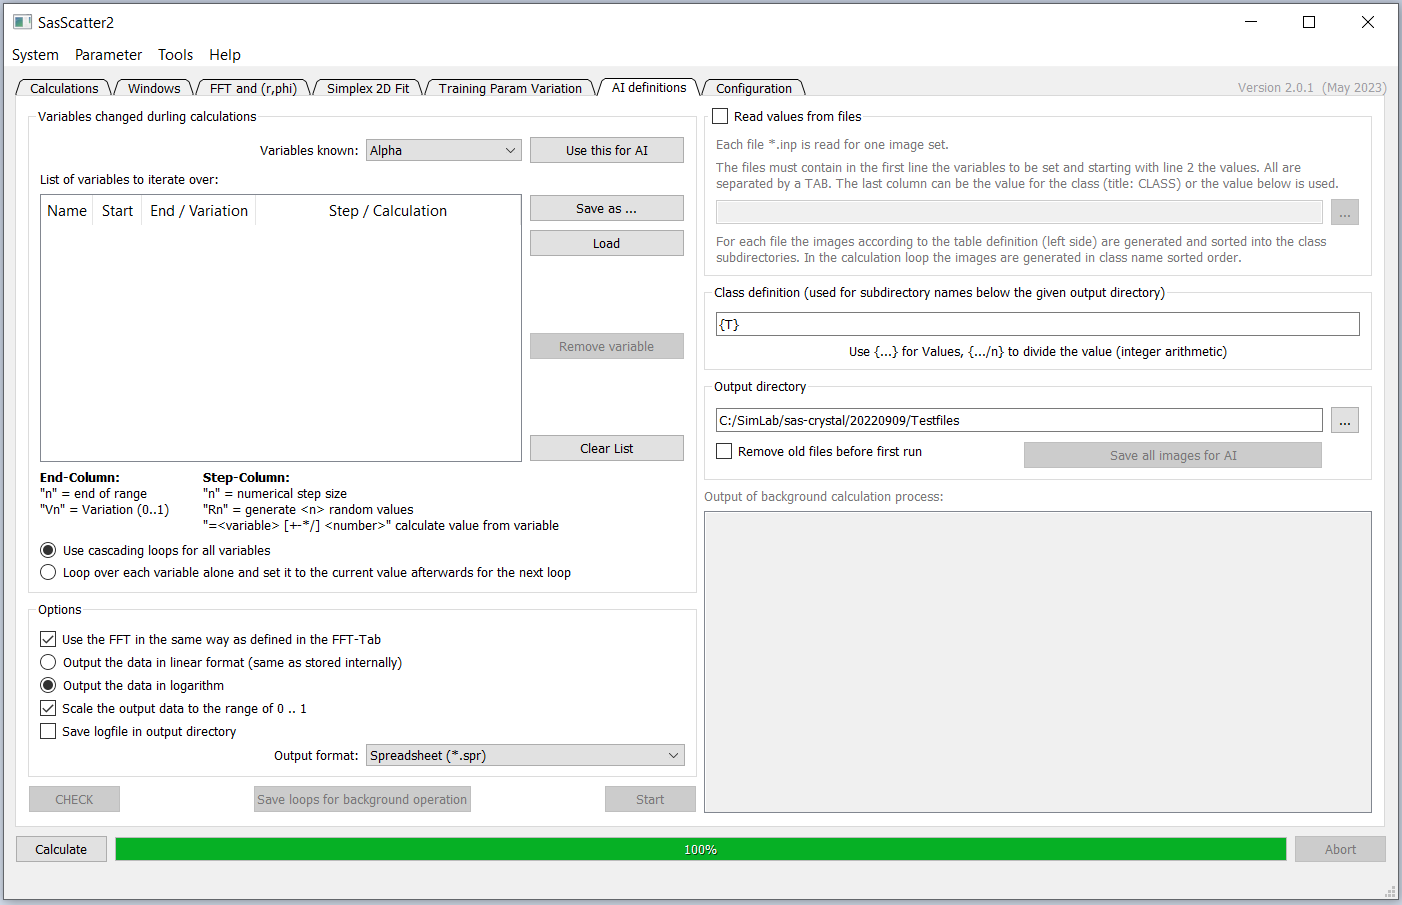
\includegraphics[width=\textwidth]{gui-aidef.png}
 \caption{AI sequence definitions}
\end{figure}

In this tab you can define how a sequence of images will be generated as a training set for a tensorflow neural network with the goal to identify some informations in real measurement data.

The usage might sound a bit complicated. Here I'll describe the input fields, the basic usage is described in a later chapter.
\begin{itemize}\itemsep0pt
\item[-] Left part from top to bottom:
\item The variable section shows all parameters to be modified during the generation. The exact usage is described in a later chapter.
\item In the option section you can enable the FFT postprocessing and modify the image output formats.
\item Button {\it CHECK} will check the processing loops and gives an information about how many images and classes will be generated.
\item Button {\it Save loops for background operation} will save the processing informations into a special file which can be read in with the console version of this program to run the calculations without a GUI in the background.
\item Button {\it Start} will start the processing directly: the special file will be generated and the background process is started. From now on you have no control over the background process except of the output shown in the list on the lower right.
\item[-] Right part from top to bottom:
\item The {\it Read values from files} option can be used to read a list of files (e.g. with different orientation vectors) and for each file the processing defined on the left side is done.
\item The {\it Class definition} is used as the subdirectory name and as a result information for the tensowflow neural network.
\item The {\it Output directory} will be populated with all generated files. it might be a good idea to remove the old imagefiles before processing starts. If you want to have more files because some parameters are randomly generated, then you can leave the old files.
\item With {\it Save all images for AI} will save all open image windows in the directory ``files/'' under the output directory in the same format as the other images will be generated. This is usefull for testing the neural network.
\item The output of the background process is shown in this list.
\end{itemize}




\subsubsection{Chatbot}
\begin{figure}[H]
 \centering
 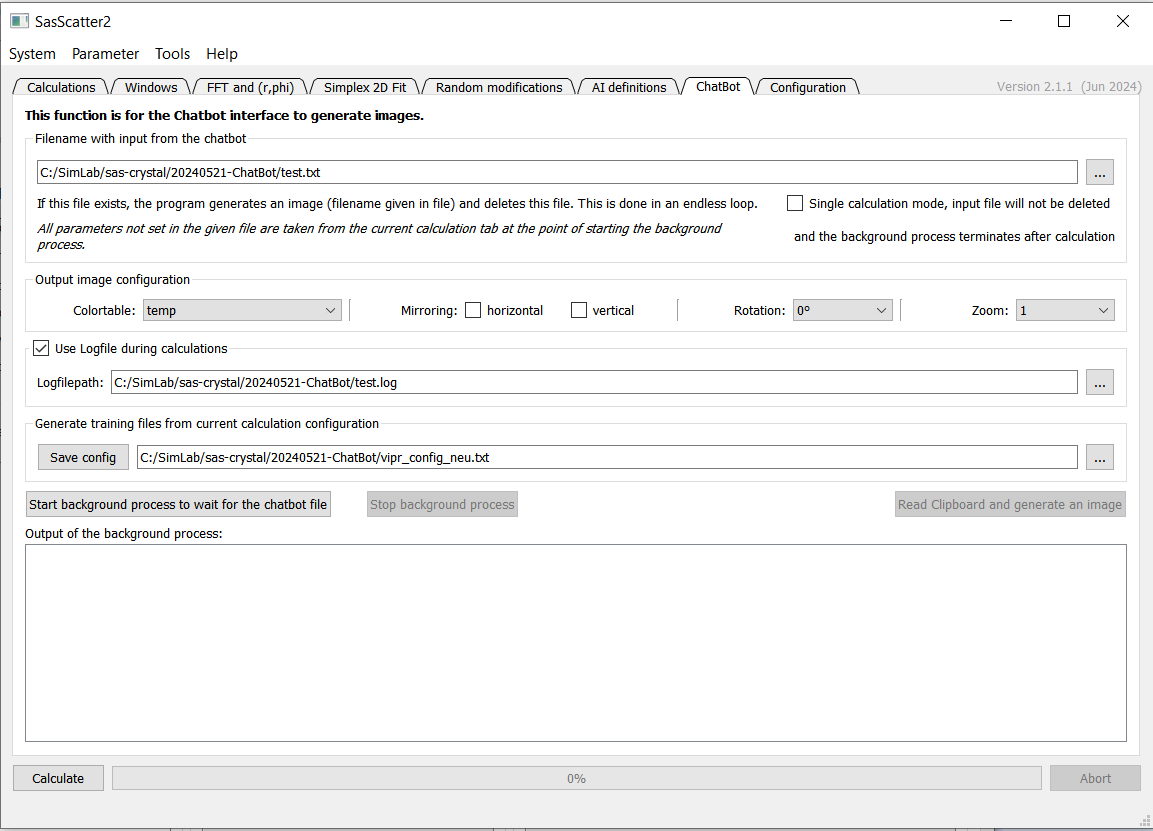
\includegraphics[width=\textwidth]{gui-chatbot.png}
 \caption{Chatbot options}
\end{figure}

Some work in the SimLab delas with a chatbot interface for this program. The idea of the usage was, that the background process started in this tab looks for a special file, read it, calculates an image, save this as a png file and then remove the input file and wait again.

The parts of this tab are:
\begin{itemize}\itemsep0pt
\item {\it Filename with inputs from the chatbot} - this is the file the background process looks for. The checkbox {\it Single calculation mode} is more for debug reasons. If checked at start of the background process, it will exit after the calculation and will  not remove the input file.
\item {\it Output image configuration} - these settings can be modified in the GUI in each image window. To generate allways the same images, you can modify them here.
\item {\it Use logfile during calculations} - if checked the given file is used to save some informations from the background process. These are not the same as displayed in the box at the bottom of this tab.
\item {\it Generate training files} - this generate a training file from the current calculation parameters. The file will be appended each time the {\it Save config} button will be pressed. This file will be use to train the chatbot to learn the parameters.
\item The buttons {\it Start} and {\it Stop} manipulates the background process.
\item {\it Read clipboard} - this makes it easier to copy the relevant informations from the chatbot interface to be used by this program. Normally you have to save the chatbot output to a special file (see above). With this you copy the text into the clipboard and click on this button to perform the calculation.
\end{itemize}
The background process is the console version of this program described later with some special parameters.



\subsubsection{Configuration}
\begin{figure}[H]
 \centering
 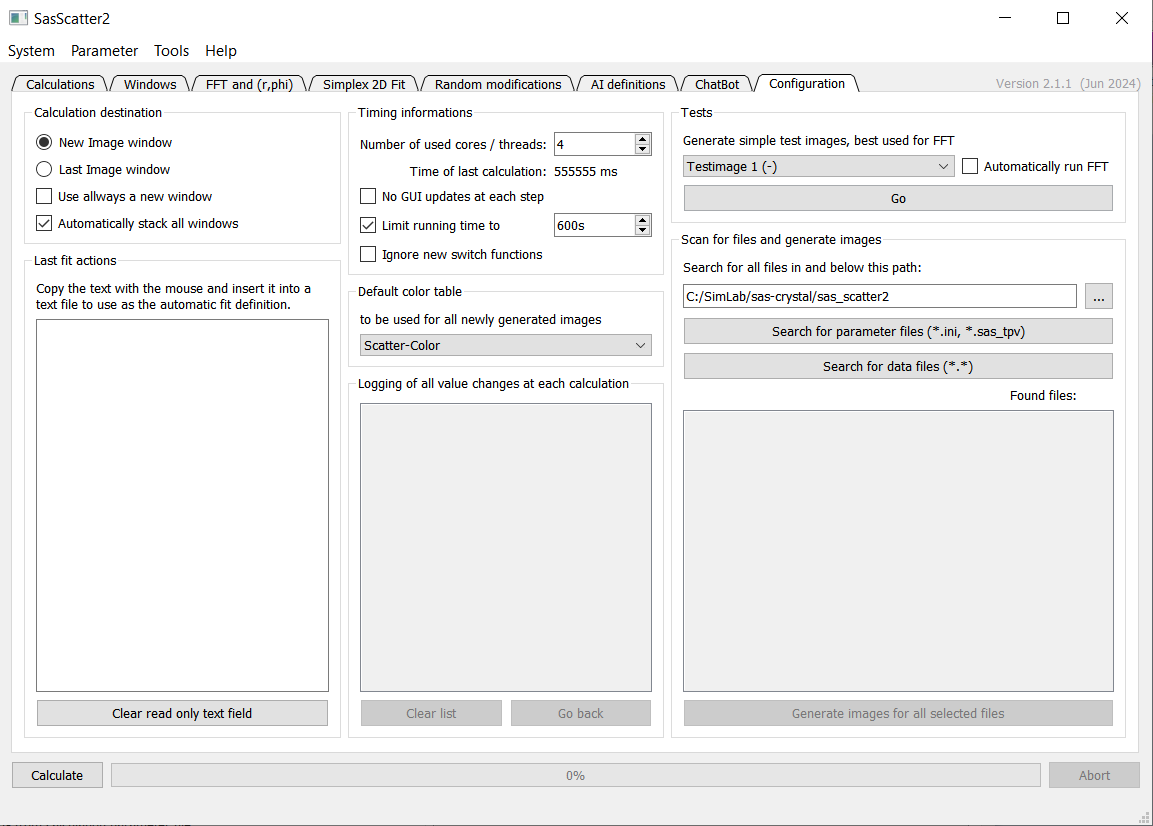
\includegraphics[width=\textwidth]{gui-config.png}
 \caption{Configuration options}
\end{figure}

\begin{itemize}\itemsep0pt
\item Group {\it Calculation destination} \\
	Here you can select the destination of the next calculated image (a new window or the last used one). This is the same information as in the Calculation tab. \\
	If the checkbox {\it Use allways a new window} is checked, then the above selected destination is ignored and each calculated image is placed in a new image window. To visualize this, the selections above and on the Calculation tab are disabled. \\
	If the checkbox {\it Automatically stack all windows} is checked, then each new image window is placed at the right side of the last one. If the screen is filled horizontally, the next row will be started below the images. If the screen is vertically filled, the program restarts at the top. But then you might have trouble to find the correct image.
\item Group {\it Last fit actions} \\
	In this text field the program writes all actions performed in the Simplex 2D Fit tab. This is useful, if you want to perform an automatic fit to get the correct syntax and to replay what you've done before. With the button under the text field you can clear this readonly field.
\item Group {\it Timing informations} \\
	Here the used number of threads (or 0 for GPU) can be set. {\bf Imoprtant note:} if a parameter set is loaded and the file contains a number of threads but a GPU is available, the GPU is selected. On the other hand, if the parameter file wants to use the GPU but currently no one avaliable, the maximum number of threads are used. \\
	The time of the last calculation is shown at the status bar for a few seconds but shown here until the next calculation overwrites it. \\
	Disabling the GUI updates might speed up the calculation time if working over the network (via ssh and vpn). \\
	The calculation time limit (if enabled) can be set to a number of seconds. After this time the calculation thread is stopped and the image displayed contains the values up to this time, the rest of the data is zero. This is the same procedure used by the Abort button (see Calculation tab).
\item Group {\it Default color table} \\
	All image windows will start with this color table. Inside each of the image windows you can change the color table independently.
\item Group {\it Logging of all value changes at each calculation} \\
	this was an idea not implemented yet.
\item Group {\it Tests} \\
	Here you can generate some special test images to check the FFT calculations. It was implemented during the FFT programming but now it's seldom used.
\item Group {\it Scan for files an generate images} \\
	You can search the given path and all subdirectories for parameter or data files. In the list of found files you can select all or some and then generate png images from the parameter or data files. The images are stored in the same location with the same name as the input file, the file extension will be png.
\end{itemize}


\subsection{Image windows}

Each calculated image or loaded dataset is displayed in a single window with some visual manipulation functions. In the title bar of the image window only a number is displayed. Just above the colorbar is the word Image and the comment field from the Calculation tab to have more informations on the image.
\begin{wrapfigure}{l}{0.36\textwidth}
  \begin{center}
    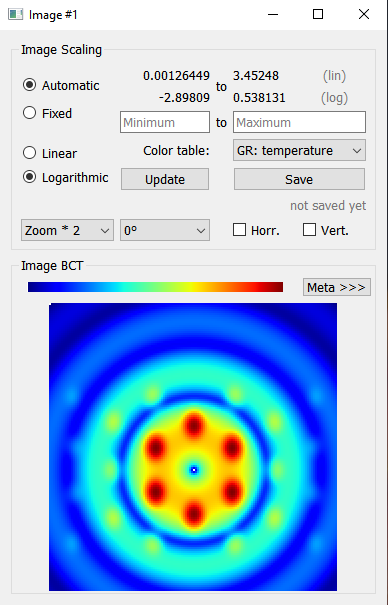
\includegraphics[width=0.35\textwidth]{img-bct.png}
  \end{center}
 \caption{Example image}
 \label{fig:img1}
\end{wrapfigure}
Select the scaling method: {\it Automatic} searches the minimal and maximal value and divide this range by the number of colors in the color table. {\it Fixed} uses the values from the input fields. To make it easier to set the same scaling in different windows, the current min/max values are displayed for the linear mode (e.g. real data values) and for the logarithmic mode (the log of the min/max data values if they are not zero or negative). Then you can select the color table scaling: {\it Linear} or {\it Logarithmic}.

You can select one of the implemented color tables. For the information which color is the min and which is the max, the colorbar is displayed just above the image.

You can set the zoom factor (no zoom, *2, *4, /2, /4), the rotation of the display and the horizontal or vertical mirroring. None of the manipulations will change the internal dataset, it affects only the visible representation.

After each change of the color table, scaling, rotation or mirroring, you have to click on the update button to update the image. Only the zoom factor generates directly a new image.

The save button saves the image in three formats: as an image (*.png), importable into Excel (*.csv) and in binary format (*.dat). The metadata is stored in a simple textfile (*.txt). After saving the path and filename is displayed just below the save button.

The Meta button will show the table of all stored metadata informations on the right side of the window (see figure \ref{fig:imagemeta}). For calculated images, the metadata contains all parameters. For loaded datasets the metadata contains all known header informations. Below this table a small histogram of the data is displayed. This histogram is calculated from the image, not from the real data. The vertical scaling is calculated from the second highest count value divided by the used 60 pixel.
\begin{figure}[H]
 \centering
 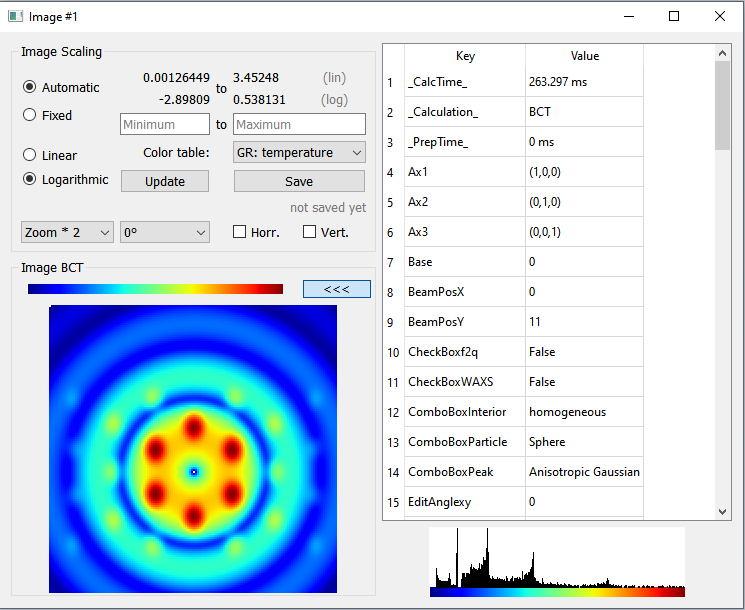
\includegraphics[width=0.67\textwidth]{img-bct-meta.png}
 \caption{Example image with meta data table}
 \label{fig:imagemeta}
\end{figure}


\subsection{Time test dialog}

\begin{wrapfigure}{r}{0.36\textwidth}
  \begin{center}
    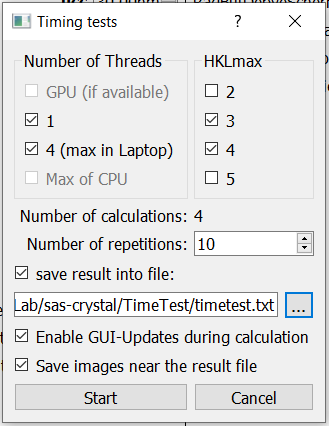
\includegraphics[width=0.3\textwidth]{timing_test.png}
  \end{center}
 \caption{Timinig test definition}
% \label{fig:timetest}
\end{wrapfigure}

This function allows the user to make a simple test of the performance of the current used system.

In the shown dialog the number of used threads are selectable, 1 thread is the slowest, 4 threads are the maximum on my development system (used for comparison), the maximum number of threads are determined by the program. The GPU can be enabled too. If not more than 4 threads possible or if no GPU found, then the apropriate checkboxes are disabled. The value of HKLmax can be set to different values, higher values increases the calculation time. If you want, you can also make the calculations for different quadrants.

The {\it New switch selection} was inserted to check the differences in internal code optimization. The old one use only the generic calculation function. The new one use special optimized functions for some of the combobox selections. So it might be a little bit faster. But at the moment not all combinations of the comboboxes are implemented as optimized functions. If one combination is not available, the generic function is used in both options.

The program calculates an image with the current parameter settings for each of the combination Quadrants/HKLmax/Threads in this loop order. The images are only saved if the apropriate checkbox is checked. The saved image files have the naming syntax: {\it timetest-t={\bf 1}-hkl={\bf 3}-q={\bf 2}.png}. No imagefiles are deleted before the test starts!

This calculations are repeated the given number of repetitions and then the minimal, maximal and mean time are saved to the given result file. During the calculations the current step is shown in the status bar.

The enabling of the GUI updates (progress bar) might increase the calculation time if you are working over the network.

The result file is written to be inserted into a \LaTeX\  {\it longtable} for documentation, the first line will contain the given comment from this dialog, the second line contains the filename with the path of the loaded parameter set (displayed here as dots because it's too long). These two lines are preceeded with a \% to make it a comment. The third line is the header of the table. This output file is {\bf not} deleted before the test starts, the new informations are allways appended.

This example screenshot calculates an fcc oriented image with a tested parameterset on my development laptop, the (Prep) means the preparation time used before the image calculation starts. In the output images below you can see the problem if not the full image is calculated and the beam center is not set to zero (e.g. the center of the image).

\begin{lstlisting}[frame=single, xleftmargin=1cm, xrightmargin=1cm]
% FCC oriented test
% Loaded parameter: ......
Threads & HKLmax & Quadrants & Min/ Mean/ Max (Prep) in ms
1 & 2 & 1 & 123.129/ 129.887/ 130.652 (2.666)
4 & 2 & 1 & 53.066/ 57.207/ 60.561 (5.288)
1 & 3 & 1 & 319.651/ 323.717/ 334.147 (6.718)
4 & 3 & 1 & 124.626/ 131.775/ 148.569 (7.258)
1 & 4 & 1 & 674.448/ 681.158/ 690.692 (7.619)
4 & 4 & 1 & 246.263/ 252.238/ 257.892 (6.815)
1 & 2 & 2 & 250.305/ 256.148/ 259.587 (6.214)
4 & 2 & 2 & 96.619/ 103.450/ 106.578 (4.733)
1 & 3 & 2 & 644.596/ 653.068/ 663.572 (5.487)
4 & 3 & 2 & 236.113/ 242.242/ 248.326 (5.410)
1 & 4 & 2 & 1348.724/ 1359.301/ 1369.582 (5.743)
4 & 4 & 2 & 485.170/ 493.482/ 505.259 (6.258)
1 & 2 & 4 & 514.255/ 519.609/ 530.854 (5.216)
4 & 2 & 4 & 206.111/ 217.372/ 235.348 (5.439)
1 & 3 & 4 & 1300.060/ 1310.465/ 1328.503 (6.104)
4 & 3 & 4 & 479.837/ 491.578/ 500.522 (6.556)
1 & 4 & 4 & 2720.594/ 2749.159/ 2879.959 (7.311)
4 & 4 & 4 & 978.576/ 1004.270/ 1046.256 (6.628)
\end{lstlisting}
\begin{figure}[H]
 \centering
 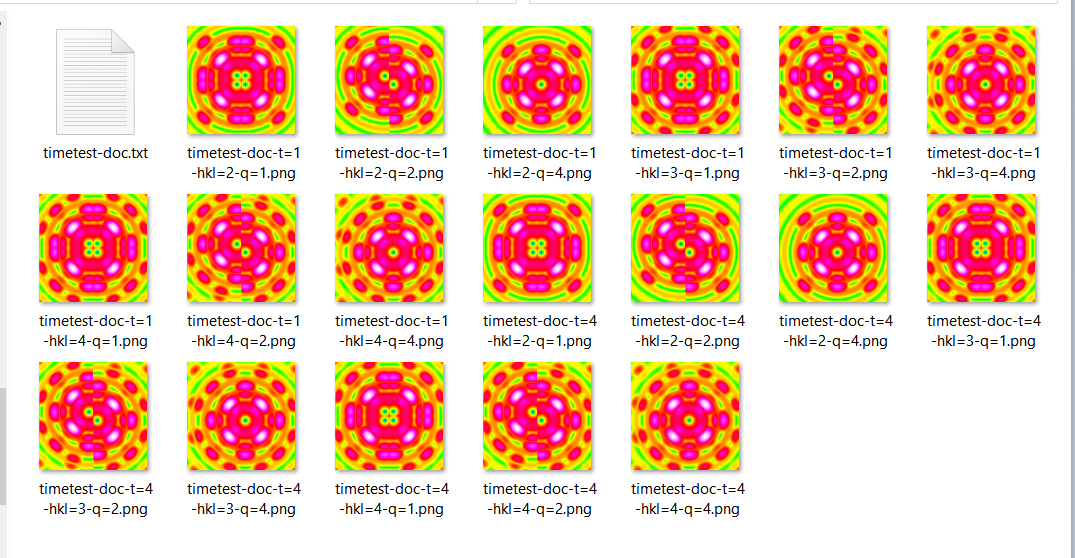
\includegraphics[width=0.85\textwidth]{timing_test_out.png}
 \caption{Output directory content after the shown test}
 \label{fig:imagemeta}
\end{figure}



%------------------------
\clearpage
\section{Usage and hints}

In these chapters I'll write some informations for the usage of the program.

\subsection{Normal image calculation}

The normal work is very easy: select the lattice type and particle information, this enables or disables other input fields. Then set the parameters to values you want and press the Calculate button. The bar right of the button shows the progress, it can be very fast. After the calculation the image will be displayed in a new window. Then you can change some parameters and recalculate the image.

\subsection{Working with measurement datasets}

Click on the {\it open data file} button in the upper left corner of the Calculation tab. You can open different file types (selected by the file extension):
	\begin{itemize}\itemsep0pt
	\item TIFF-Images (*.tif *.tiff), multiple images are not recognized in the current version
	\item KWS-Data (*.dat *.data)
	\item ESRF/Klora images (*.edf), might be very large
	\item Spreadsheet-Format (*.spr)
	\item 2D SANS (*.xml *.csv *.dat)
	\item SasCrystal (*.dat *.csv *.txt), the local format if images are saved
	\item[] {\it If the HDF5 library is included:}
	\item HDF5 Files (*.h5 *.hdf *.hdf5 *.nxs), if more than one image is found, a selection dialog will ask the user which image(s) should be loaded and displayed. If used in the automatic fit, only the first selected image will be used. {\it The meta data usage is under development.}
	\end{itemize}
Each data file will be opened in a new window. And the internal flag is set so that the next calculated image will be opened in an other new window. The main goal is to use the measurement data for the 2D Fit.
%\begin{figure}[H]
% \centering
% 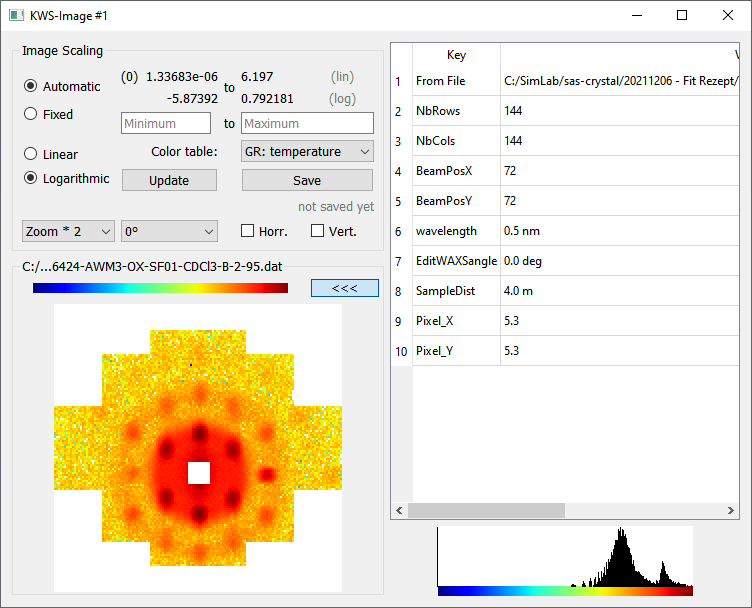
\includegraphics[width=0.67\textwidth]{img-kwsdata-meta.png}
% \caption{Example KWS image with meta data table}
%\end{figure}

\subsection{Working with the Simplex 2D Fit}

The implemented Downhill Simplex Algorithm can be used to calculate the parameters to generate an image fitted to the given dataset.

\subsubsection{Manual mode}

The manual fit mode is used to get an idea of some fit parameters. And you can obtain some fit steps to put them later into an automated procedure.

At every fit step you have to think about the variables (which you want to be modified, what is the starting value and what are the limits). Then press the {\it Start 2d-Fit} button. The progress of the fit will be documented in the list box on the right side. At the end the Result column of the variable table will be filled. For the next fit run press the button {\it Fit Result Use it} to copy the result values as the new start values and press the start button again.

If you want to see the result image click on the calculate button (lower left) to get a new or update the last image window. Be sure to klick on the button {\it Fit Result Use it} before calculation.

\subsubsection{Automatic mode}

If you use the manual fit mode, each fit step will be written in the text field in the configuration tab in the syntax to be used for the automatic mode. These steps can be copied into a file to be used as an input for this mode.

The possible commands (at the beginning of each line) for this automatic mode input file are:
\begin{itemize}\itemsep0pt
\item {\bf \#} this line is a comment and will be ignored, empty lines are ignored too.
\item {\bf EOF} \\
	This ends the file. The other way was to comment out the rest of the file, but this is more complicated.
\item[] {\it The following commands are only interpreted during the first scan of the file. More scans are done if more than one input file is included.}
\item {\bf Scale:} {\it $<$Min$>$, $<$Max$>$} \\
	This sets the scaling for all images to the given values. Otherwise each fit image will get the scaling from its original image and this ist set to local min/max.
\item {\bf GlobLog:} {\it filename} \\
	The given filename is used for the global logfile. If \LaTeX\  output is enabled, the path is used for this output file, the name is fixed to \path{latex-output.tex}.
\item {\bf Param:} {\it filepath} \\
	The parameter input file to be used during the fit as a first start.
\item {\bf DirMask:} {\it *.dat} \\
	Filemask used for the DirUp / DirDown commands.
\item {\bf DirUp:} {\it dir} \\
	Directory to be scanned in alphanumeric ascending order.
\item {\bf DirDown:} {\it dir} \\
	Directory to be scanned in alphanumeric descending order.
\item {\bf File:} {\it filepath} \\
	Single file to be used (multiple occurances possible).
\item {\bf Limits:} {\it $<$Parametername$>$; $<$Min$>$; $<$Max$>$} \\
	Set the limits used during the fit for the given parameter (multiple occurances possible).
\item[] {\it The following commands are interpreted at every file scan.}
\item {\bf Info:} {\it informational text} \\
	This text will be shown in the GUI, more than 20 chars can disturb the GUI layout.
\item {\bf Use:} {\it $<$Param1$>$, $<$Param2$>$, ... } \\
	List of parameternames used during the next fit step.
\item {\bf Fit:} {\it Stp=3.0; Iter=20; Tol=0.0010; Diff$<$5} \\
	Perform one fit operation. The values of Stp (Step size), Iter (Maximum iterations), Tol (Tolerance) are the same as in the GUI used for this fit run. After each fit run the percentual change of each parameter is summed up and if this sum is less than the Diff value the fit step is finished. If not, this fit run is repeated up to 20 times to avoid endless loops.
\end{itemize}


%\clearpage
%\subsection{Generate AI files}
%
%I've played around with some neural networks to find some parameters automatically. For this I used a docker image with a preinstalled tensorflow system. The goal was to train this network with as many images as possible to get a good result.
%
%\subsubsection{Example to use the AI files}



%------------------------
\clearpage
\section{Console version}

To perform the calculation work in a batch job, the console version of the program was written. It was only a wrapper around the same calculation routines as the GUI version. It has no GUI but a lot of calling arguments to configure the calculations. The call is: \\
\centerline{{\bf sas\_scatter2Cons} {\it options and parameters}}

\begin{longtable}{|L{1cm}|L{2cm}|C{2cm}|L{12cm}|}
\caption{Possible options for sas\_scatter2Cons} \\
\hline\rowcolor{rowcolor}{\bf Short} & {\bf Long} & {\bf Parameter} & {\bf Description} \\
\endfirsthead
\hline\rowcolor{rowcolor}{\bf Short} & {\bf Long} & {\bf Parameter} & {\bf Description} \\
\endhead
\hline
-h & -{}-help & & Displays help on commandline options. \\ \hline
 & -{}-help-all & & Displays help including Qt specific options. \\ \hline
-v & -{}-version & & Displays version information. \\ \hline
-p & -{}-paramfile & {\it paramfile} & Filepath loaded as the parameter set for all calculations (*.ini). \\ \hline
-c & -{}-seqfile & {\it aifile} & Filepath loaded as the AI definition sequence (*.sas\_airun). \\ \hline
-i & -{}-img & {\it imgfile} & Filepath and name to save the image (*.png). Or the image to load for automatic fit (*.dat). \\ \hline
-t & -{}-threads & {\it threads} & Number of threads used (default=max cores), set to {\bf 0} to use GPU if available. \\ \hline
-l & -{}-logfile & {\it logfile} & Filepath and name of the logfile for informations of the process (*.log). \\ \hline
 & -{}-csv & {\it csvfile} & Filepath and name of the csvfile for some statistic outputs during 2D-Fit (*.csv). \\ \hline
-f & -{}-autofit & {\it autofit} & Filepath and name for the automatic fit routine (*.txt). If this is given, the AI-File is ignored and the imagefile is an input dataset. \\ \hline
-o & -{}-output & {\it output} & Filepath and name of the single output image of the automatic fit routine or the path to save the  multifile outputs. \\ \hline
 & -{}-nofft & & If set, the FFT calculation during AI generation is skipped. \\ \hline
 & -{}-noconsole & & If set, no output is printed to the console during auto fit (except statistic info). \\ \hline
 & -{}-swap & {\it [HV]} & Set the image swapping and can contain the characters 'H' and/or 'V'. \\ \hline
 & -{}-rotate & {\it [0123]} & Set the image ratoation to 0(=0°), 1(=90°), 2(=180°), 3(=270°). \\ \hline
 & -{}-zoom & {\it [124]} & Set the image zoom factor to 1, 2, 4. \\ \hline
 & -{}-color & {\it color} & Set the used colortable to one of: grey, glow, earth, temp. \\ \hline
 & -{}-tpv & {\it file} & Inputfile (*.sas\_tpv) for the train parameter variation section to generate a number of random modified datasets (incl. r,phi and fft images). This parameter can be given more than once. If this is the last parameter, a wildcard for the filename can be used too. \\ \hline
 & -{}-tpvimg & {\it number} & Number of images to generate, will overwrite the factor value in the *.sas\_tpv files. \\ \hline
 & -{}-timetest & {\it filename} & Start timing test. No output image is generated. Use -o to set the generated output file with the statistics and -p for the parametr file for the calculation. The given config file can be generated with the GUI and contains the test definitions. \\ \hline
 & -{}-chatbot & {\it filename} & The program waits for the given input file (generated from a chatbot), calculates and saves the image and removes the input file. \\ \hline
 & -{}-cbkeep & & If set, the inputfile is kept and the program ends after one calculation. This is useful during debugging, not needed in normal operations. \\ \hline
\end{longtable}




\end{document}
